\documentclass[11pt, class=article, crop=false]{standalone}
\usepackage[subpreambles=true]{standalone}
\usepackage[T1]{fontenc} % for font setting
\usepackage{newtxtext,newtxmath}
\usepackage{import,
            graphicx,
            parskip,
            url,
            amsmath,
            wrapfig,
            fancyhdr,
            soul,
            tabularx,
            authblk,
            textcomp,
            lineno}

% side caption figure
\usepackage{sidecap}
\sidecaptionvpos{figure}{t}

% for special characters in bibliography            
\usepackage[utf8]{inputenc}
\usepackage[T1]{fontenc}

% citation setup
\usepackage[euler]{textgreek}
\usepackage[sort\&compress]{natbib}
\usepackage[utf8]{inputenc}
\setcitestyle{square}
\setcitestyle{comma}
\bibliographystyle{vancouver}

% caption setup
\usepackage[font = small, labelfont = {bf, small}]{caption}
           
% margin
\usepackage[top=2.54cm, bottom=2.54cm, left=2.54cm, right=2.54cm]{geometry}

% title
\title{Appendix}
\date{} % remove date from title

% author list
\author{}
%\author[1]{Ashley LaRoque}
%\author[2]{Seoghyun Kim}
%\author[1]{Akira Terui}
%\affil[1]{Depatment of Biology, University of North Carolina at Greensboro}
%\affil[2]{Department of Biological Sciences, Kangwon National University}

\begin{document}

\renewcommand{\theequation}{S\arabic{equation}}
\renewcommand{\thetable}{S\arabic{table}}
\renewcommand{\thefigure}{S\arabic{figure}}

\maketitle

\tableofcontents

\newpage

\section{Detection Model}

Our capture-recapture data was collected seasonally and fish may be subject to different detection probabilities by season.
As such, accounting for detection probabilities is essential to obtain reliable estimates of fish density.
We utilized a spatial Cormack-Jolly-Seber (CJS) model \citep{schaubEstimatingTrueInstead2014} to account for seasonal detection probabilities. 
This model allowed us to estimate seasonal detection probabilities while accounting for permanent emigration and survival.

\textit{Observation process} -- 
We assumed that the recapture state $Y_{j,t}$ for unique individual $j$ at occasion $t$ ($Y_{i,t} = 1$ if recaptured, $0$ otherwise) is a random draw from a Bernoulli distribution:

\begin{equation}
    Y_{j,t} \sim \text{Bernoulli}(p_{i,t} r_{j, t} z_{j,t}),
\end{equation}

where $p_{j,t}$ is the detection probability, $r_{j, t}$ is the binary latent variable indicating the survival state of individual $j$, and $z_{j, t}$ is the binary latent variable indicating whether individual $j$ remained in the study section.

Our primary interest was to estimate seasonal detection probabilities.
We allowed $p_{j, t}$ to vary by season in a logit scale:

\begin{equation}
    \text{logit}~p_{j,t} = \mu_p + \alpha_p Q_{t},
\end{equation}

where $Q_{t}$ is a dummy variable discerning winter (coded as 0: November -- February) and summer (coded as 1: May -- August).
This formulation translates into the winter detection as $p_{\text{win}} = \text{inv.logit}(\mu_p)$ and the summer detection as $p_{\text{sum}} = \text{inv.logit}(\mu_p + \alpha_p)$

% Our ability to detect individuals that have remained within the study section is partially dependent on seasonal changes such as day length and temperature.
% Therefore, we accounted for this difference in our detection probability $p_{i,t}$ across individuals $i$ and occasions $t$ using a logit-link function:

% \begin{equation}
%     \text{logit}(Ym_{i, t}) \sim \mu \alpha Sm_{i, t}
% \end{equation}

% where $\mu$ is the prior for recapture, $\alpha$ is the prior that accounts for the seasonal effect, and $Sm$ is the seasonal index broken into two components (0 = winter, 1 = summer). 

\textit{State process} -- 
Our model accounted for survival and movement processes to obtain less biased estimates of detection probabilities.
The survival state in the (spatial) CJS model conditions on the first capture of individual $j$.
Let $f_{j}$ denote the first capture occasion for individual $j$.
Then,

\begin{align}
    \begin{split}
        r_{j, f_j} &= 1,\\
    r_{j, t + 1} | r_{j, t} &\sim \text{Bernoulli}(r_{j,t} s_{j,t}),    
    \end{split}
\end{align}

where $s_{j,t}$ is the survival probability between $t$ and $t + 1$.
Since our interest was to estimate detection probabilities, we made a simplifying assumption on the survival probability as $s_{j, t} = \psi^{\eta_{j,t}}$, where $\psi$ is the daily survival probability and $\eta_{j,t}$ is the interval (unit: day) between occasion $t$ and $t + 1$.

We also accounted for emigration.
Let $X_{j, t+1}$ and $X_{j, t}$ denote locations of recapture at occasion $t+1$ and capture at occasion $t$ for unique individual $j$, which were measured as the distance from the midpoint of the section to the downstream end of the study stretch.
As in the main text, we assumed $X_{j,t+1}$ as a random draw from a normal distribution conditional on the capture location $X_{j,t}$ as:

\begin{align}
    \begin{split}
        X_{j, t+1}|X_{j, t}, \sigma_{j, t} &\sim \text{Normal}(X_{j, t}, \sigma_{j, t}^2)\\
        \ln \sigma_{j, t} &= \ln \sigma_0 + \ln \eta_{j, t}
    \end{split}
    \label{eq:si-normal}
\end{align}

where $\sigma_0$ is the standard deviation describing the daily distance moved between occasion $t$ and $t+1$ and $\eta_{j,t}$ is the interval (unit: day) between the occasions for individual $j$.
Unlike the main movement model, we were unable to include predictors for $\sigma_{j,t}$ since predictor values were unavailable when individual $j$ was not recaptured.

The latent variable $z_{j,t}$ was determined by the observed (if recaptured) or predicted location (if not recaptured) of unique individual $j$ as: 

\begin{equation}
    z_{j,t} =
    \begin{cases}
        1~\text{if}~0 \le X_{j,t} \le L~\text{(stay)},\\
        0~\text{otherwise (emigrate)}.
    \end{cases}
\end{equation}

$L$ is the upstream terminal of the study reach ($L = 430$).
When $X_{j, t+1}$ was unobserved (i.e., not recaptured), a predicted value was drawn from Equation \ref{eq:si-normal} through the Markov Chain Monte Carlo simulations.

% \textit{Survival probability}- Individuals must survive from the previous occasion in order to possibly be recaptured. To estimate the probability $\phi$ of an individual $i$ surviving to occasion $t$, the following is assumed:

% \begin{equation}
%     \text{logit}(\phi.day_{i, t}) \sim \mu_\phi
% \end{equation}

% where the survival probability per day $\phi.day$ is described using a logit-link function. Here, $\mu_\phi$ is the prior for survival. This is used to described the cumulative probability of survival $\phi$ using a log-link function: 

% \begin{equation}
%     \text{log}(\phi_{i, t}) \sim Int_{i, t} \text{log}(\phi.day_{i, t})
% \end{equation}

% where $Int_i,t$ is the time interval between capture and recapture in accordance with log-transformed survival per day $\phi.day_{i, t}$.

The model was fitted to the data for each species separately using JAGS \citep{plummerJAGSProgramAnalysis2003}. Vague or weakly informative priors were used for parameters: $\text{Unif}(0, 1)$ for survival probability $s_{j,t}$, and $\text{Normal}(0, 10^2)$ for the seasonal effect $\alpha_p$ and the daily movement parameter $\ln \sigma_0$. Markov chain Monte Carlo (MCMC) simulations were run for 20,000 iterations with a 1,000 burn-in period and we retained 1,000 samples per chain by thinning every 40 steps to calculate posterior probabilities. Model convergence was checked by ensuring that the potential scale reduction factor, referred to as R-hat, was less than 1.1 for all parameters. All statistical analyses were conducted in R version 4.4.0 \citep{rcoreteamLanguageEnvironmentStatistical2021}. 

Estimated detection probabilities were summarized in Table \ref{tab:detection}. We calculated the corrected density $N_{\text{cor}}$ as $N_{\text{cor}} = N_{\text{obs}}p_{\text{sum}}^{-1}$ for summer months and $N_{\text{cor}} = N_{\text{obs}}p_{\text{win}}^{-1}$ for winter months, where $N_{\text{obs}}$ is the observed fish density. $N_{\text{cor}}$ was used as predictors in our movement model in the main text.

\newpage

% \section{Figures}

% \subsection{Figure S1 Abundance of all captured fish species}

% \begin{figure}
%     \centering
%     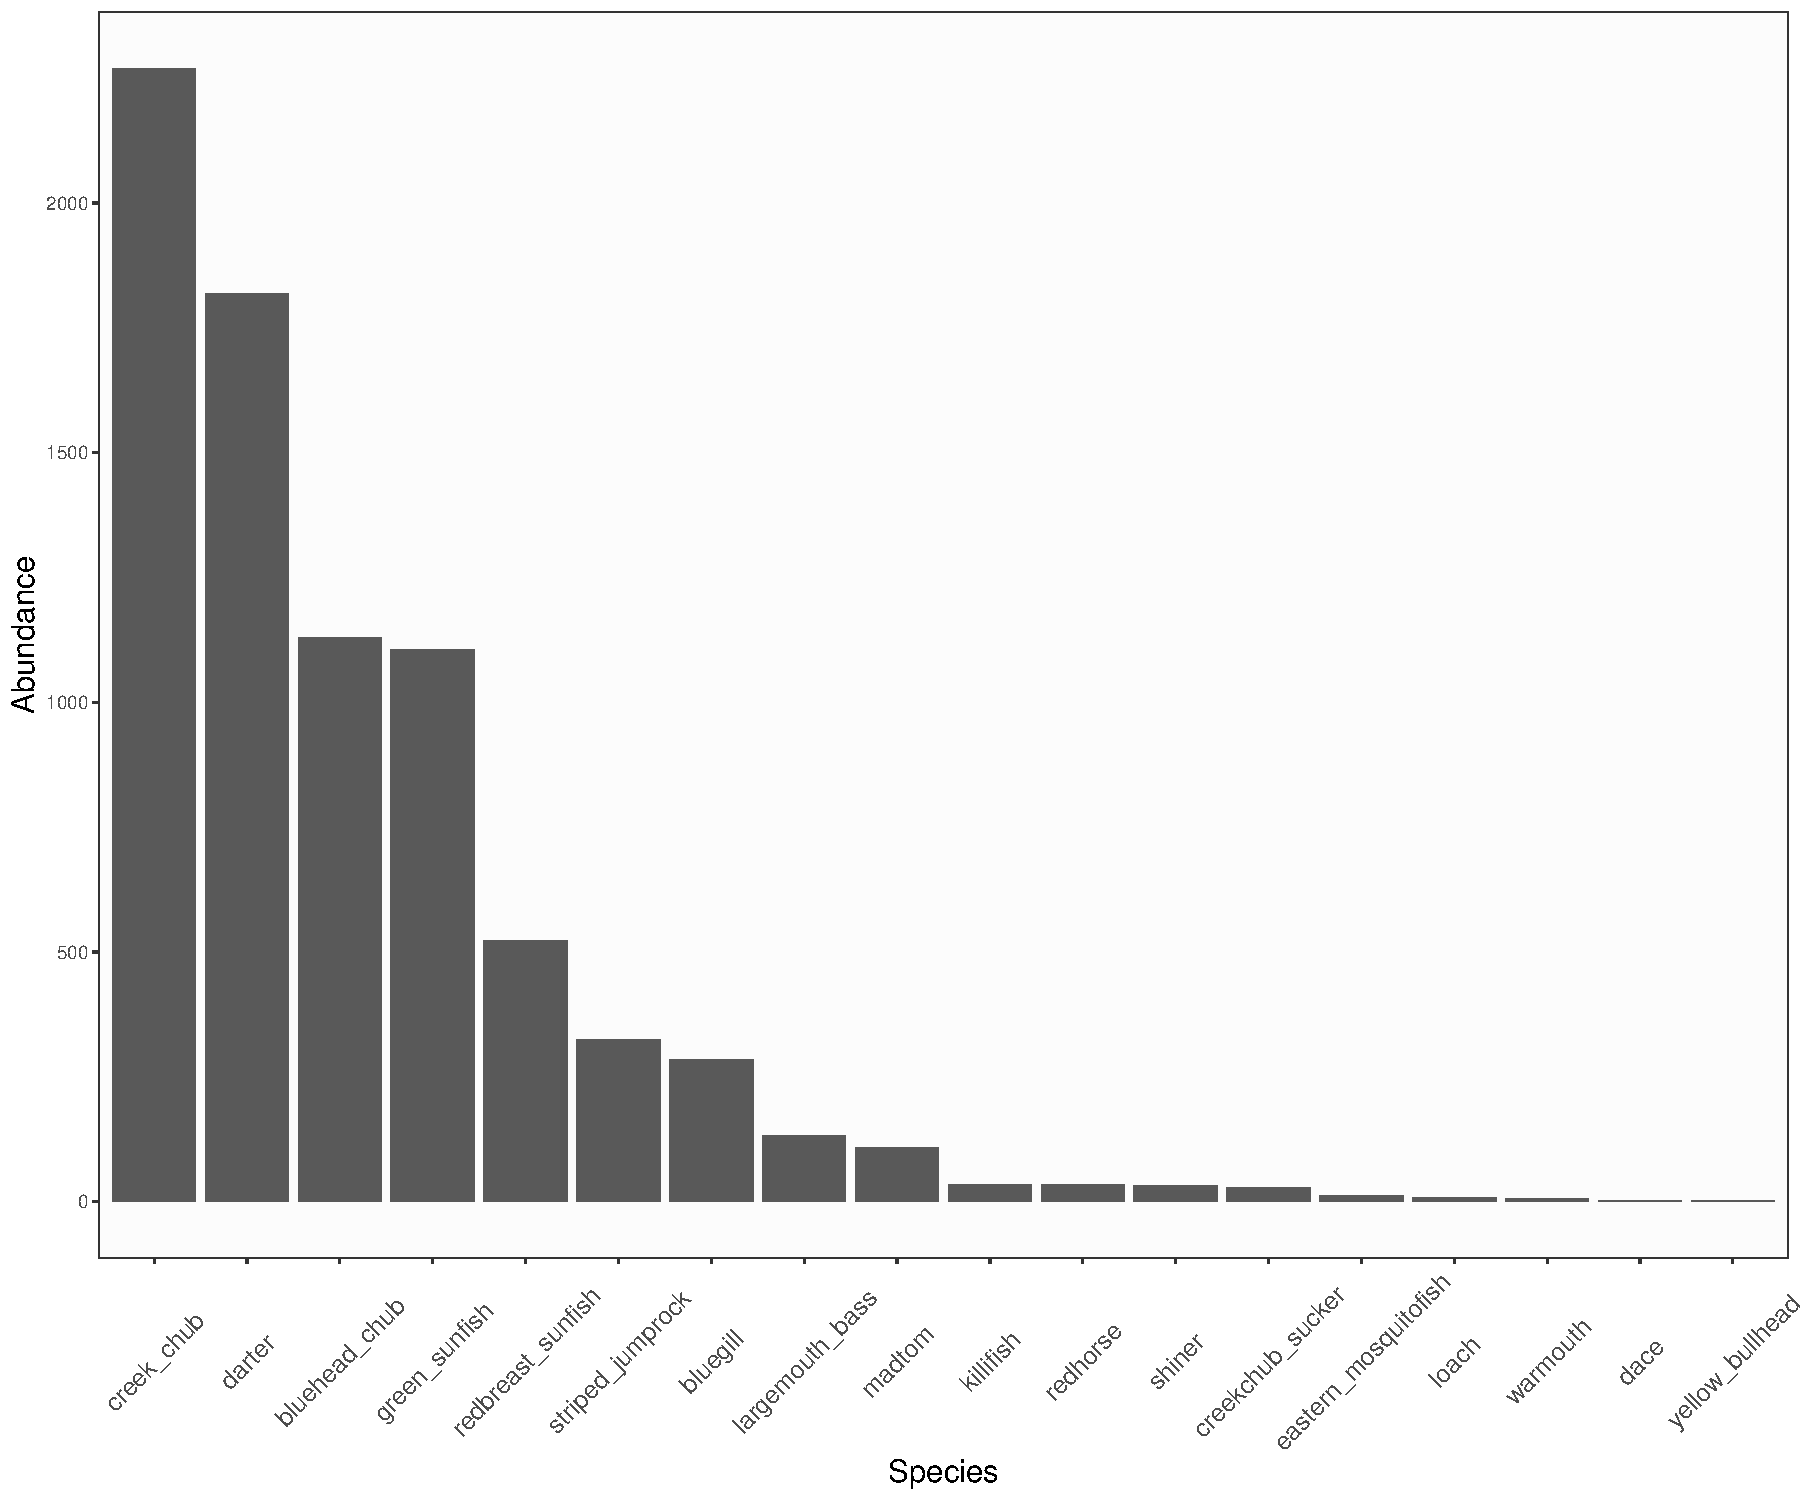
\includegraphics[width=0.9\linewidth]{output/fig_abundance.pdf}
%     \caption{Abundance (n) of each species collected during backpack electrofishing ordered from most to least abundant.}
%     \label{fig:fig_abundance}
% \end{figure}

% \newpage

% \subsection{Figure S2 Median length at capture of tagged species}

% \begin{figure}
%     \centering
%     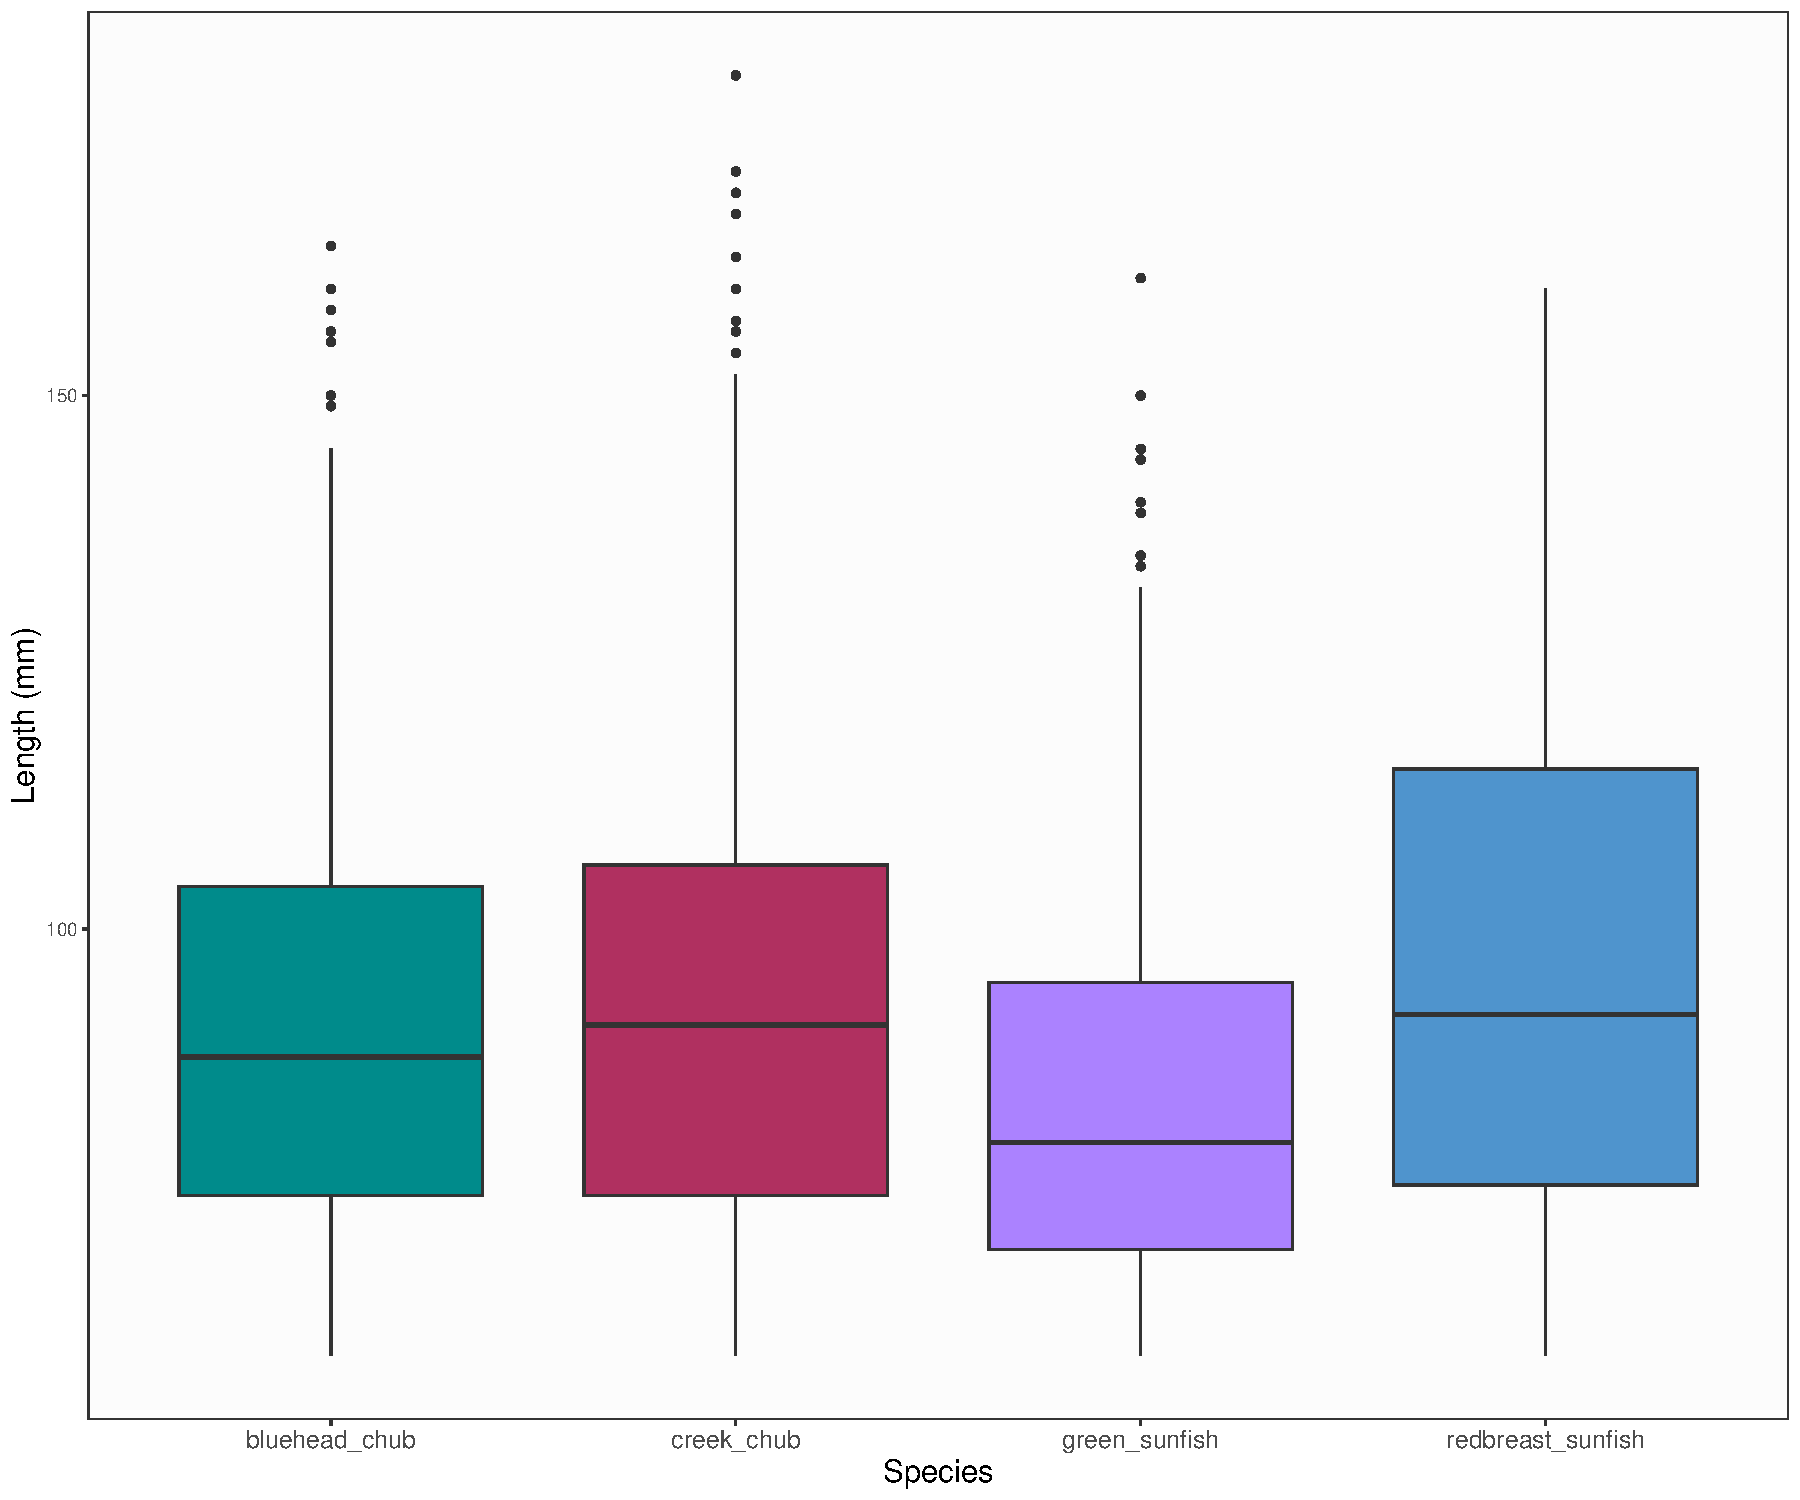
\includegraphics[width=0.9\linewidth]{output/fig_size_dist.pdf}
%     \caption{Median length at initial capture for each target species described by the solid black line within the boxplot. The interquartile range is depicted by the size of each box and colored by species. Outliers are shown as points.}
%     \label{fig:fig_size_dist}
% \end{figure}

% \newpage

% \subsection{Figure S3 Absolute movement by each species per season}

% \begin{figure}
%     \centering
%     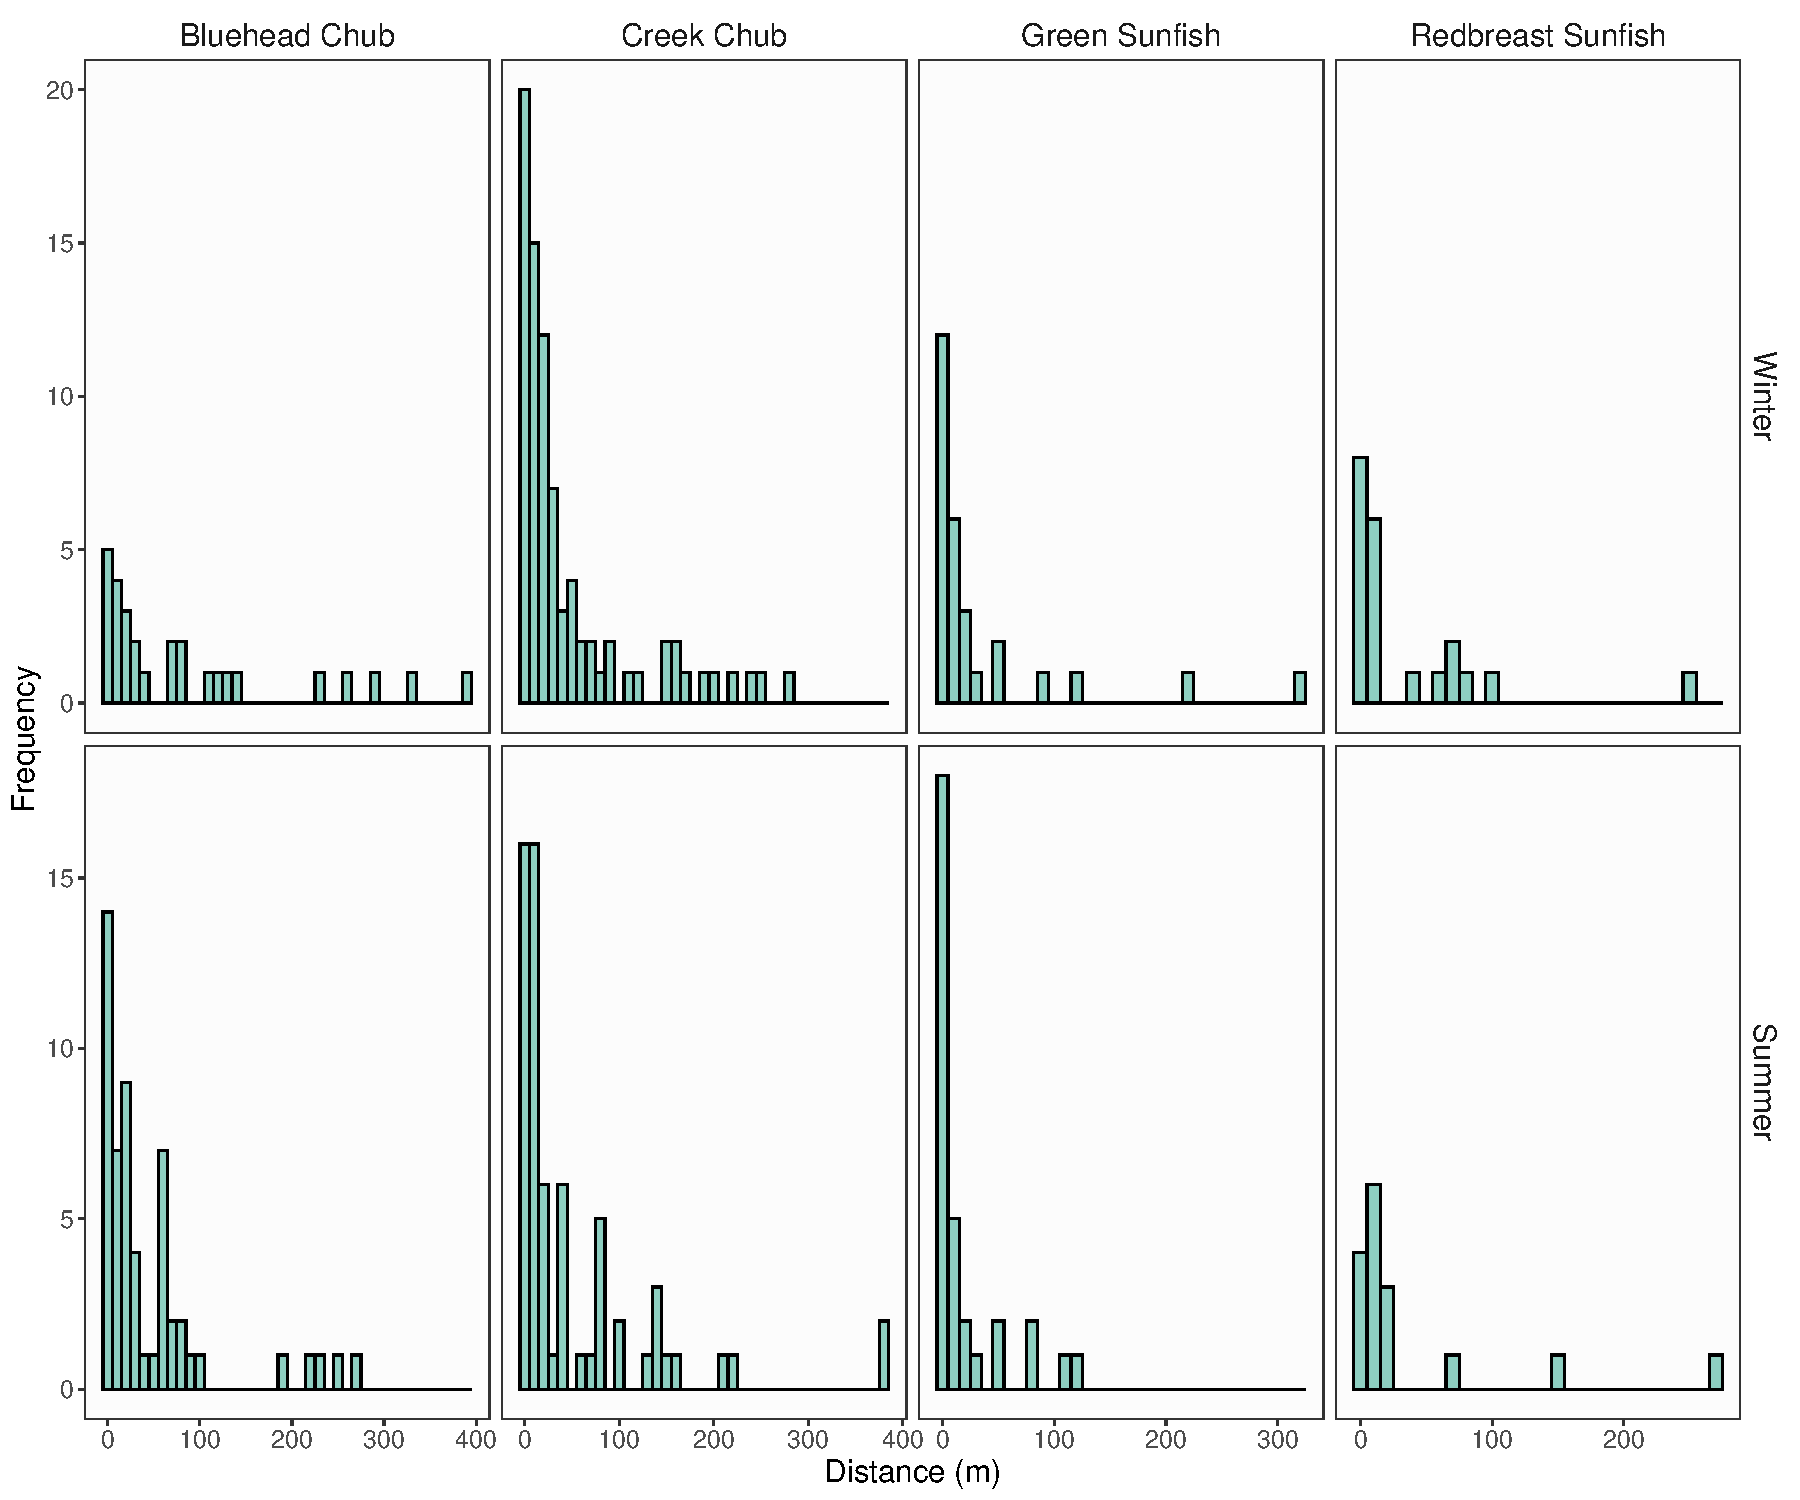
\includegraphics[width=0.9\linewidth]{output/fig_total_move.pdf}
%     \caption{The frequency of total absolute movement for each target species shown for both winter and summer seasons.}
%     \label{fig:fig_total_move}
% \end{figure}

% \newpage

\section{Tables}

\subsection*{Seasonal detection probabilities}

\begin{table}[ht]
\centering
\caption{Seasonal detection probabilities estimated by the spatial CJS model.} 
\label{tab:detection}
\begin{tabular}{lll}
  \hline
Species & Season & Estimate \\ 
  \hline
Bluehead chub & Winter & 0.23 [0.18 - 0.30] \\ 
   & Summer & 0.32 [0.25 - 0.41] \\ 
  Creek chub & Winter & 0.25 [0.20 - 0.31] \\ 
   & Summer & 0.35 [0.28 - 0.44] \\ 
  Green sunfish & Winter & 0.13 [0.09 - 0.18] \\ 
   & Summer & 0.21 [0.15 - 0.27] \\ 
  Redbreast sunfish & Winter & 0.12 [0.07 - 0.21] \\ 
   & Summer & 0.29 [0.19 - 0.41] \\ 
   \hline
\end{tabular}
\end{table}


\newpage

\subsection*{Number of unique and replicate capture and recaptures}

% latex table generated in R 4.4.1 by xtable 1.8-4 package
% Wed Oct 22 14:46:46 2025
\begin{table}[ht]
\centering
\caption{The number of unique individuals, unique recaptures, captured replicates (including multiple captures of the same individual), and recaptured replicates (including multiple recaptures of the same individual) listed from left to right for each target species.} 
\label{tab:capture}
\scalebox{0.8}{
\begin{tabular}{lrrrr}
  \hline
Species & Unique & Unique Recaptures & Replicate Captures & Replicate Recaptures \\ 
  \hline
Bluehead chub & 479 &  73 & 615 &  82 \\ 
  Creek chub & 1191 & 111 & 1391 & 145 \\ 
  Green sunfish & 503 &  56 & 612 &  60 \\ 
  Redbreast sunfish & 257 &  33 & 317 &  37 \\ 
   \hline
\end{tabular}
}
\end{table}


\newpage

\subsection*{Mean and standard deviation of total length}

% latex table generated in R 4.4.1 by xtable 1.8-4 package
% Thu Jun 26 12:25:29 2025
\begin{table}[ht]
\centering
\caption{Mean and standard deviation total length (mm) for each target species.} 
\label{tab:size}
\begin{tabular}{lrr}
  \hline
Species & Mean & Standard Deviation \\ 
  \hline
Bluehead chub & 91.41 & 21.02 \\ 
  Creek chub & 92.38 & 21.10 \\ 
  Green sunfish & 84.59 & 18.43 \\ 
  Redbreast sunfish & 96.17 & 24.37 \\ 
   \hline
\end{tabular}
\end{table}


\newpage

\subsection*{Mean and standard deviation of species density}

% latex table generated in R 4.4.1 by xtable 1.8-4 package
% Wed Oct 22 14:46:45 2025
\begin{table}[ht]
\centering
\caption{Mean and standard deviation of detection-corrected density ($\n/m^2$) of each target species.} 
\label{tab:density}
\begin{tabular}{lrr}
  \hline
Species & Mean & Standard Deviation \\ 
  \hline
Bluehead chub & 0.31 & 0.34 \\ 
  Creek chub & 0.62 & 0.56 \\ 
  Green sunfish & 0.51 & 0.50 \\ 
  Redbreast sunfish & 0.29 & 0.49 \\ 
   \hline
\end{tabular}
\end{table}


\newpage

\subsection*{Movement model coefficients}

\small
{\begin{table}[ht]
\centering
\caption{Parameter estimates of the movement model. Median estimates and their associated posterior probabilities are reported.} 
\label{tab:coefficients}
\begin{tabular}{llrrr}
  \hline
Species & Effect & Estimate & Pr(< 0) & Pr(> 0) \\ 
  \hline
Bluehead chub & Intercept & -0.22 & 0.86 & 0.14 \\ 
   & ln(Body length) & -0.04 & 0.57 & 0.43 \\ 
   & Habitat refuge area & -0.03 & 0.57 & 0.43 \\ 
   & Current velocity & 0.01 & 0.49 & 0.51 \\ 
   & Temperature & -0.35 & 0.97 & 0.03 \\ 
   & Density bluehead chub & 0.01 & 0.47 & 0.53 \\ 
   & Density creek chub & 0.01 & 0.48 & 0.52 \\ 
   & Density green sunfish & -0.17 & 0.84 & 0.16 \\ 
   & Density redbreast sunfish & 0.06 & 0.34 & 0.66 \\ 
   & Recapture probability & 0.19 & 0.00 & 1.00 \\ 
   & d.f. in t distribution & 3.32 & 0.00 & 1.00 \\ 
  Creek chub & Intercept & -0.74 & 1.00 & 0.00 \\ 
   & ln(Body length) & 0.35 & 0.02 & 0.98 \\ 
   & Habitat refuge area & 0.07 & 0.28 & 0.72 \\ 
   & Current velocity & -0.09 & 0.84 & 0.16 \\ 
   & Temperature & -0.08 & 0.70 & 0.30 \\ 
   & Density bluehead chub & -0.15 & 0.92 & 0.08 \\ 
   & Density creek chub & 0.12 & 0.19 & 0.81 \\ 
   & Density green sunfish & 0.20 & 0.10 & 0.90 \\ 
   & Density redbreast sunfish & -0.08 & 0.68 & 0.32 \\ 
   & Recapture probability & 0.13 & 0.00 & 1.00 \\ 
   & d.f. in t distribution & 3.14 & 0.00 & 1.00 \\ 
  Green sunfish & Intercept & -2.14 & 1.00 & 0.00 \\ 
   & ln(Body length) & 1.76 & 0.00 & 1.00 \\ 
   & Habitat refuge area & -0.58 & 0.98 & 0.02 \\ 
   & Current velocity & -0.08 & 0.67 & 0.33 \\ 
   & Temperature & -0.08 & 0.62 & 0.38 \\ 
   & Density bluehead chub & -0.95 & 1.00 & 0.00 \\ 
   & Density creek chub & 0.84 & 0.00 & 1.00 \\ 
   & Density green sunfish & -0.27 & 0.83 & 0.17 \\ 
   & Density redbreast sunfish & 0.46 & 0.04 & 0.96 \\ 
   & Recapture probability & 0.13 & 0.00 & 1.00 \\ 
   & d.f. in t distribution & 3.08 & 0.00 & 1.00 \\ 
  Redbreast sunfish & Intercept & -0.33 & 0.91 & 0.09 \\ 
   & ln(Body length) & -0.30 & 0.90 & 0.10 \\ 
   & Habitat refuge area & -0.58 & 0.96 & 0.04 \\ 
   & Current velocity & -0.38 & 0.99 & 0.01 \\ 
   & Temperature & -0.13 & 0.73 & 0.27 \\ 
   & Density bluehead chub & -0.48 & 0.99 & 0.01 \\ 
   & Density creek chub & 0.42 & 0.02 & 0.98 \\ 
   & Density green sunfish & -0.35 & 0.92 & 0.08 \\ 
   & Density redbreast sunfish & 0.20 & 0.17 & 0.83 \\ 
   & Recapture probability & 0.17 & 0.00 & 1.00 \\ 
   & d.f. in t distribution & 41.75 & 0.00 & 1.00 \\ 
   \hline
\end{tabular}
\end{table}
}

% \newpage
% \subsection{Table S5 Mean and standard deviation of habitat variables}

% % latex table generated in R 4.4.1 by xtable 1.8-4 package
% Wed Oct 22 14:46:50 2025
\begin{table}[ht]
\centering
\caption{Mean and standard deviation across sections and occasions for each habitat variable.} 
\label{tab:habitat}
\begin{tabular}{lrr}
  \hline
Habitat Metric & Mean & Standard Deviation \\ 
  \hline
Mean Section Area (m$^2$) & 32.51 & 9.21 \\ 
  Pool Area (m$^2$) & 18.60 & 17.14 \\ 
  Riffle Area (m$^2$) & 4.84 & 8.35 \\ 
  Run Area (m$^2$) & 9.07 & 11.21 \\ 
  Habitat Refuge Area (m$^2$) & 0.45 & 0.84 \\ 
  Mean Depth (cm) & 18.78 & 10.31 \\ 
  Section Length (m) & 9.94 & 1.07 \\ 
  Mean Substrate (mm) & 4.20 & 1.42 \\ 
  Mean Velocity (m/s) & 0.06 & 0.08 \\ 
  Mean Width (m) & 3.26 & 0.82 \\ 
  Mean Temperature (C) & 14.58 & 6.27 \\ 
   \hline
\end{tabular}
\end{table}


\newpage

\bibliography{tex/references}

\end{document}
